% Autor: Leonhard Segger, Alexander Neuwirth
% Datum: 2017-10-30
\documentclass[
	% Papierformat
	a4paper,
	% Schriftgröße (beliebige Größen mit „fontsize=Xpt“)
	12pt,
	% Schreibt die Papiergröße korrekt ins Ausgabedokument
	pagesize,
	% Sprache für z.B. Babel
	ngerman
]{scrartcl}

% Achtung: Die Reihenfolge der Pakete kann (leider) wichtig sein!
% Insbesondere sollten (so wie hier) babel, fontenc und inputenc (in dieser
% Reihenfolge) als Erstes und hyperref und cleveref (Reihenfolge auch hier
% beachten) als Letztes geladen werden!

\usepackage{tikz}
\usetikzlibrary{backgrounds,calc,patterns,angles,quotes} % loads some tikz extensions\usepackage{tikz}
\usetikzlibrary{babel}
% Silbentrennung etc.; Sprache wird durch Option bei \documentclass festgelegt
\usepackage{babel}
% Verwendung der Zeichentabelle T1 (Sonderzeichen etc.)
\usepackage[T1]{fontenc}
% Legt die Zeichenkodierung der Eingabedatei fest, z.B. UTF-8
\usepackage[utf8]{inputenc}
% Schriftart
\usepackage{lmodern}
% Zusätzliche Sonderzeichen
\usepackage{textcomp}

% Mathepaket (intlimits: Grenzen über/unter Integralzeichen)
\usepackage[intlimits]{amsmath}
% Ermöglicht die Nutzung von \SI{Zahl}{Einheit} u.a.
\usepackage{siunitx}
% Zum flexiblen Einbinden von Grafiken (\includegraphics)
\usepackage{graphicx}
% Abbildungen im Fließtext
\usepackage{wrapfig}
% Abbildungen nebeneinander (subfigure, subtable)
\usepackage{subcaption}
% Funktionen für Anführungszeichen
\usepackage{csquotes}
\MakeOuterQuote{"}
% Zitieren, Bibliographie
\usepackage[sorting=none]{biblatex}

%fixed die Citations in captions, die die Reihenfolge rippen
%\usepackage{notoccite}

% Zur Darstellung von Webadressen
\usepackage{url}
%chemische Formeln
\usepackage[version=4]{mhchem}
% siunitx: Deutsche Ausgabe, Messfehler getrennt mit ± ausgeben
\usepackage{floatrow}
\floatsetup[table]{capposition=top}
\usepackage{float}
% Verlinkt Textstellen im PDF-Dokument
\usepackage[unicode]{hyperref}
% "Schlaue" Referenzen (nach hyperref laden!)
\usepackage{cleveref}
\sisetup{
	locale=DE,
	separate-uncertainty
}
\bibliography{14Mo_O5_02-07-2018_References}

\begin{document}
	
	\begin{titlepage}
		\centering
		{\scshape\LARGE Versuchsbericht zu \par}
		\vspace{1cm}
		{\scshape\huge O5 - Spektrometer \par}
		\vspace{2.5cm}
		{\LARGE Gruppe 14Mo \par}
		\vspace{0.5cm}
		
		{\large Alexander Neuwirth (E-Mail: a\_neuw01@wwu.de) \par}
		{\large Leonhard Segger (E-Mail: l\_segg03@uni-muenster.de) \par}
		\vfill
		
		durchgeführt am 04.07.2018\par
		betreut von\par
		{\large Johann Preuß} 
		
		\vfill
		
		{\large \today\par}
	\end{titlepage}
	\tableofcontents
	\newpage

	\section{Kurzfassung}
	Es werden mit einem Spektrometer verschiedene Methoden der räumlichen Trennung von Wellenlängen und Spektren verschiedener Lampen untersucht.
	Zunächst wird das Spektrum einer Natriumdampflampe mit einem Prisma und zwei verschiedenen Transmissionsgittern untersucht.
	Erwartet wird hierbei, dass die verschiedenen Methoden alle zu demselben Linienmuster führen.
	Dies lässt sich nicht bestätigen, da beim Gitter für höhere Ordnungen weniger Spektrallinien gemessen werden und die Gitter leicht unterschiedliche Ergebnisse liefern.
	Es kann aber gezeigt werden, dass die qualitativen Ergebnisse des Prismas  mit den Ergebnissen der Untersuchung der Gitter in großen Teilen übereinstimmen.
	
	Weiterhin wird mithilfe des bekannten Spektrums einer Heliumlampe der Zusammenhang zwischen Wellenlänge und Beugungswinkel bestimmt und genutzt, um den Winkelmessungen der untersuchten Spektren eine Wellenlänge zuordnen zu können.
	
	Es wird das Spektrum einer Energiesparlampe gemessen.
	Dabei wird erwartet, dass sich das Spektrum eindeutig dem Emissionsspektrum eines Gases zuordnen lässt.
	Dies ist jedoch nicht der Fall.
	
	Zuletzt werden die Maxima der Spektren verschiedenfarbiger LEDs gemessen, um daraus und aus den Spannungen, ab denen die LEDs zu leuchten beginnen, das Plancksche Wirkungsquantum zu bestimmen.
	Es wird erwartet, dass das Ergebnis mit dem Literaturwert übereinstimmt, was jedoch nur innerhalb der 1,5-fachen Unsicherheit gezeigt werden kann. %182 Wörter
	
	\section{Methoden}
	
	Zunächst wird das Spektrometer gemäß dessen Anleitung justiert.
	Dabei wird der Prismentisch so ausgerichtet, dass bei Veränderung des Winkels, unter dem das Licht einfällt, die vertikale Position des Spalts im Beobachtungsfernrohr sich nicht verändert.
	Der Spalt wird so schmal gestellt, dass gerade genug Licht durchdringt, als dass er noch gut zu sehen ist.
	Eine Natriumdampflampe wird vor den Spalt gebracht und das Prisma auf den Prismentisch in den Strahlengang gestellt. 
	Durch das Fernrohr wird das Linienspektrum beobachtet und jeweils Farbe und ungefähre relative Position notiert.
	
	Dann wird das Prisma durch ein Transmissionsgitter mit $g=\SI{1/300}{mm} $ ersetzt.
	Die Winkelplatte wird so justiert, dass bei Ausrichtung des Fadenkreuzes im Fernrohr auf das Maximum nullter Ordnung ein Winkel von \SI{0}{\degree} gemessen wird.
	Dann werden für eine Drehrichtung für alle erkennbaren Spektrallinien der Winkel abgelesen und, wenn sie erkennbar ist, die Farbe der Linie notiert.
	Dasselbe wird für die erste Ordnung bei einem Gitter mit $g=\SI{1/600}{mm} $ durchgeführt.
	
	Nun wird die Natriumdampflampe durch eine Heliumlampe ersetzt.
	Für diese wird das Winkelspektrum der ersten Ordnung aufgenommen, um später anhand einer Kalibriertabelle die Abhängigkeit von Wellenlänge zu gemessenem Winkel bestimmen zu können. %Winkelspektrum? I guess...
	
	Das Spektrum einer Energiesparlampe wird bei der ersten Ordnung aufgenommen, wobei markiert wird, ob es sich um diskrete Linien oder um das Maximum eines ausgeschmierten Bereichs handelt.
	Zuletzt werden die Maxima des Spektrums von verschiedenfarbigen Leuchtdioden aufgenommen und jeweils gemessen, ab welcher Diodenspannung sie sichtbar zu leuchten beginnen.
	
	In \cref{fig_aufbau} sind das Spektrometer und die anderen Bestandteile des Versuchsaufbaus dargestellt.
	
	\begin{figure}[H] 
		\includegraphics[width=1\textwidth]{fig_aufbau}
		\centering
		\caption{Das Spektrometer und die anderen Versuchsmaterialien, die verwendet wurden. \cite{Aufbau}}
		\label{fig_aufbau}
		\centering
	\end{figure}

	\section{Ergebnisse und Diskussion}

	\subsection{Unsicherheiten}
	Die Unsicherheiten werden gemäß GUM ermittelt. 
	Außerdem wird für Unsicherheitsrechnungen die Python-Bibliothek "uncertainties" verwendet.
	\begin{description}
		\item[Winkelmessung:] Die Winkel am Spektrometer lassen sich zwar sehr präzise ablesen, aber das Einstellen des Fadenkreuzes auf die Linie war nur begrenzt präzise, da das schwarze Fadenkreuz vor dem schwarzen Hintergrund sehr schlecht zu erkennen ist.
		Demnach wird für das Ablesen des Winkels die Unsicherheit auf \SI{0,02}{\degree} abgeschätzt.
		\item[Spannungsmessung:] Die Spannung wurde am Multimeter auf zwei Nachkommastellen genau angezeigt, woraus eine Unsicherheit von \SI{0,003}{V} folgt (rechteckige WDF).
		Da die Spannung lediglich zum Messen, wann die LED zu leuchten beginnt, verwendet wurde und da das Auge nicht eine beliebig geringe Intensität zuverlässig von Null unterscheiden kann, wurde die Unsicherheit mit \SI{0,03}{V} abgeschätzt.
	\end{description}
	
	\subsection{Natriumdampflampe}
	\subsubsection{Beobachtung und Datenanalyse}
	\subsubsection*{Prisma}
	Die hinter dem Prisma erkennbaren Spektrallinien sind in \cref{fig_draw} skizziert. 
	Die Spektrallinien wurden von links nach rechts stärker gebrochen.
	Auftretende Restlichteffekte ließen sich durch Abschirmung mit beispielsweise den Händen entfernen.
	\begin{figure}[H]
		\centering
		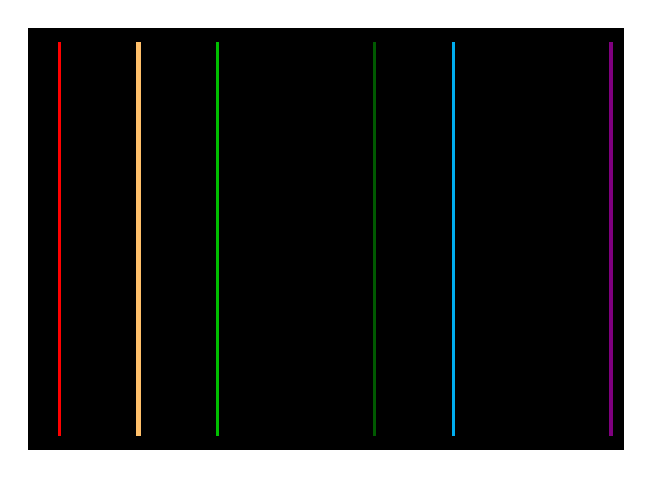
\begin{tikzpicture}[background rectangle/.style={fill=black}, show background rectangle]
			\def\len{5}
			\def\rot{10}
			\def\orange{11}
			\def\gruen{12}
			\def\dgruen{14}
			\def\tuerkis{15}
			\def\lila{17}
			\draw[-,very thick, color=red] (\rot,0) -- (\rot,\len) node [pos=.5,sloped,above] {};
			\draw[-,ultra thick, color={rgb:orange,2;yellow,2;pink,5}] (\orange,0) -- (\orange,\len) node [pos=.5,sloped,above] {};
			\draw[-,very thick, color=black!25!green] (\gruen,0) -- (\gruen,\len) node [pos=.5,sloped,above] {};
			\draw[-,very thick, color=black!65!green] (\dgruen,0) -- (\dgruen,\len) node [pos=.5,sloped,above] {};
			\draw[-,very thick, color=cyan] (\tuerkis,0) -- (\tuerkis,\len) node [pos=.5,sloped,above] {};
			\draw[-,very thick, color=violet] (\lila,0) -- (\lila,\len) node [pos=.5,sloped,above] {};
		\end{tikzpicture}
		\caption{Qualitative Skizze der sichtbaren Spektrallinien der Natriumdampflampe nach Brechung an einem Prisma. Die Abstände sind nur grob abgeschätzt.} 
		\label{fig_draw}
	\end{figure}

	\subsubsection*{Gitter}
	Die Winkel der Spektrallinien lassen sich mit der Formel aus der Einführung in Wellenlängen umrechnen:
	\begin{equation}
		\lambda = \frac{g \cdot \sin{\vartheta_m}}{m}
		\label{eq_lambda}
	\end{equation}
	\begin{equation}
		u(\lambda) = \left|\frac{g \cdot \cos{\vartheta_m} \cdot u(\vartheta_m)}{m}\right|
	\end{equation}
 	Dabei ist $g$ die Gitterkonstante und $\vartheta_m$ der Beugungswinkel des $m$-ten Beugungsmaximums.
	In \cref{fig_natrium} sind für die Gitter mit $g=1/\SI{300}{mm}$ und $g=1/\SI{600}{mm}$ die aus den Winkeln resultierenden Wellenlängen verschiedener Ordnungen dargestellt.
	
	\begin{figure}[H] 
		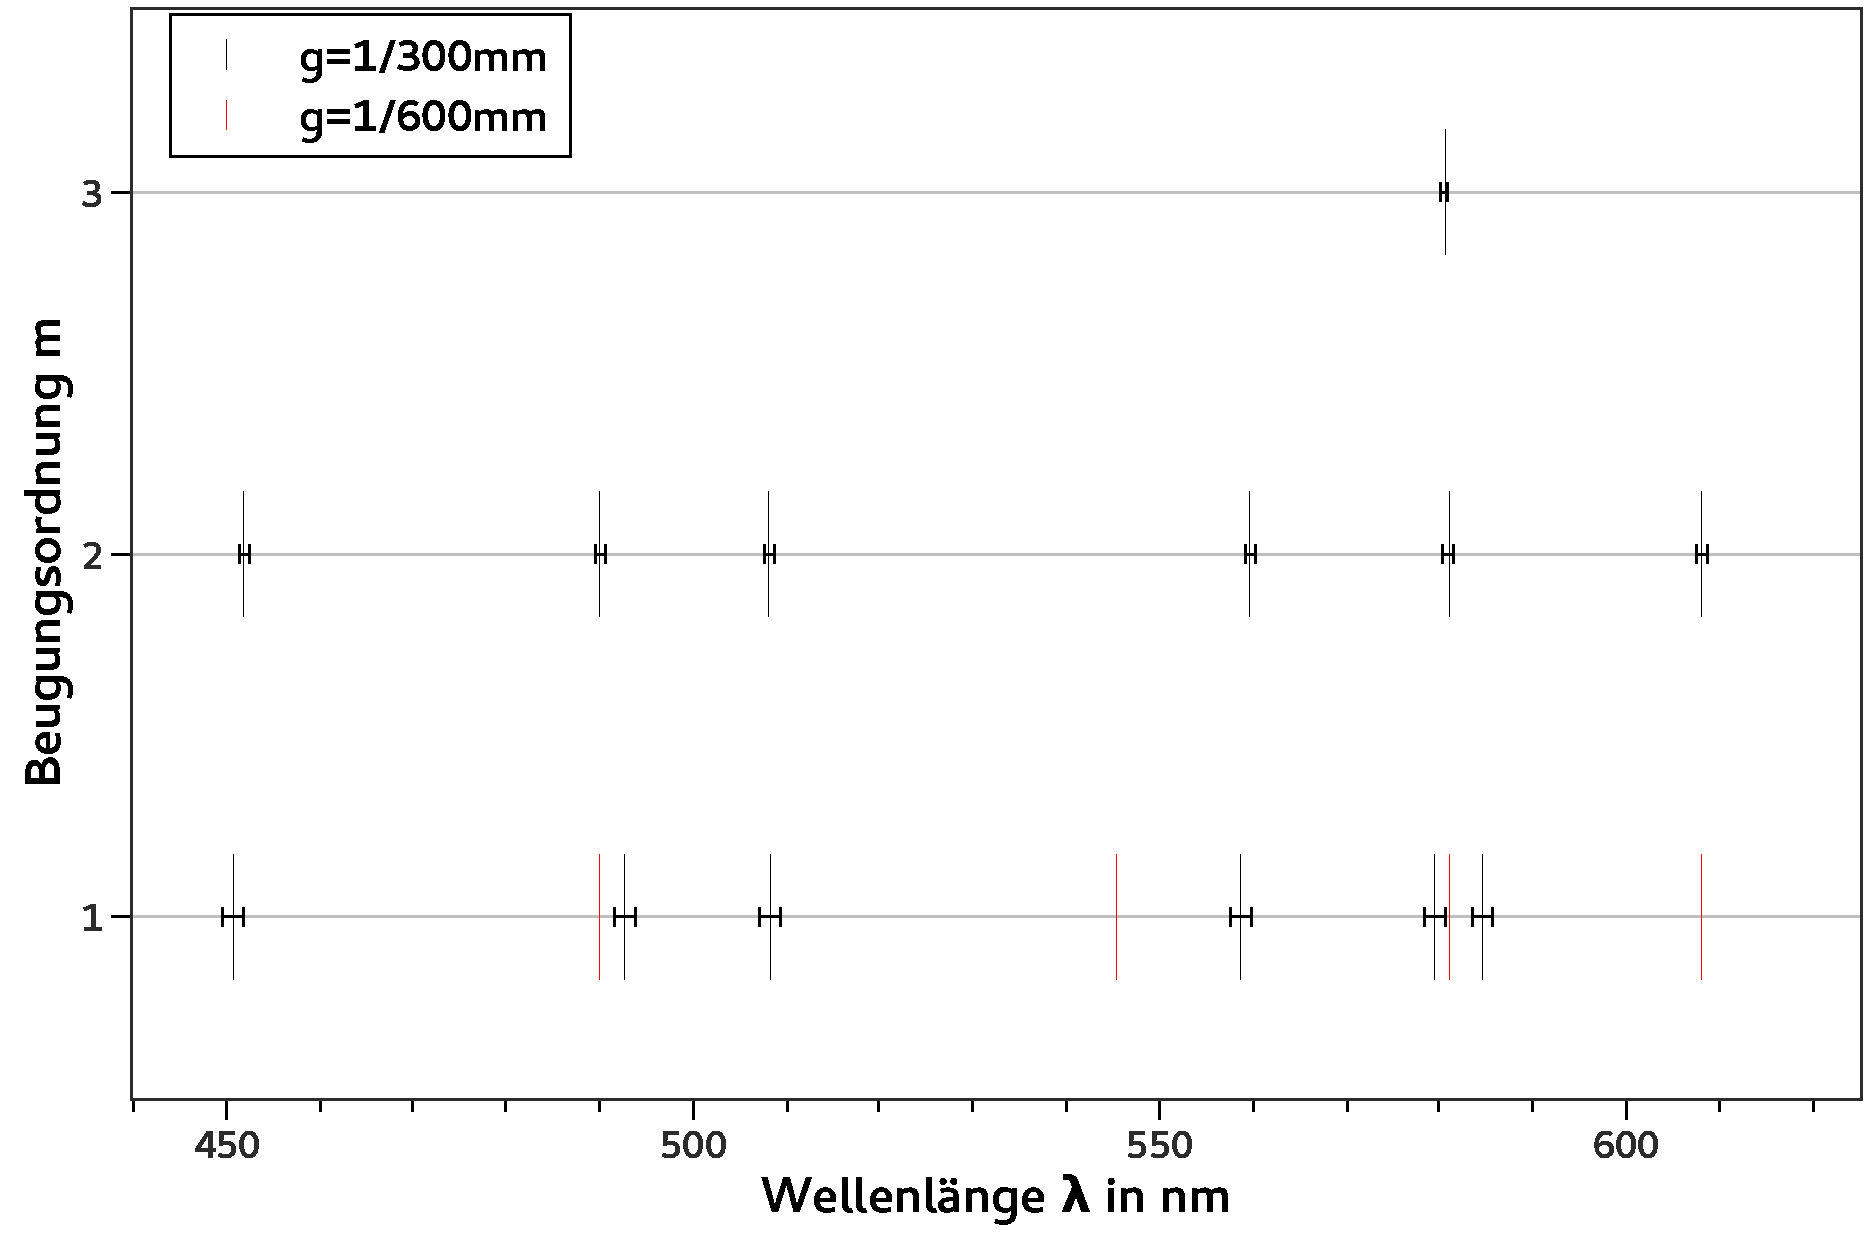
\includegraphics[width=1\textwidth]{fig_natrium}
		\centering
		\caption{Die aus dem Beugungswinkel der Maxima resultierenden Wellenlängen einer Natriumdampflampe sind abgebildet.
		In Schwarz sind die Messwerte beim Gitter mit 300 Spalten pro Millimeter dargestellt und die Rot die vom Gitter mit 600 Spalten pro Millimeter. 
		Die Unsicherheit der roten Messpunkte ist kleiner als die Symbolgröße.
		}
		\label{fig_natrium}
		\centering
	\end{figure}

	\subsubsection{Diskussion}
	
	\cite{NatriumDoppel} gibt an, dass Natrium eine doppelte sehr starke Spektrallinie, die Natrium-Doppellinie, bei \SI{589,0}{\nano \meter} und \SI{589,6}{\nano \meter} hat.
	Diese kann durch das Gitter beobachtet werden und auch durch das Prisma lässt sich eine sehr helle Spektrallinie der entsprechenden Färbung erkennen, wie in \cref{fig_natrium} zu erkennen ist.
	Sie kann jedoch in beiden Fällen und auch bei höheren Ordnungen des Gitters nicht in die beiden Teillinien aufgelöst werden.
	Dies ist nicht überraschend, da die Unsicherheit der Wellenlänge bereits größer als die Differenz der Wellenlänge der beiden Linien ist.
	Beim Vergleich der Spektrallinien in den ersten drei Ordnungen fällt zunächst auf, dass in der dritten Beugungsordnung nur noch die Natrium-Doppellinie beobachtet werden kann, was daran liegt, dass die Linien hier nur noch eine so geringe Intensität haben, dass sie mit dem bloßen Auge nicht mehr beobachtet werden können.
	Nur die intensitätsstärkste Linie wird noch gesehen.
	Der Vergleich der beiden Gittern untereinander erlaubt die Feststellung, dass die Linien teilweise beieinander liegen, aber teilweise auch Abweichungen vorhanden sind.
	Die Spektrallinie bei ca. \SI{608}{\nano \meter} konnte beim ersten Gitter nur in zweiter Ordnung gemessen werden, beim zweiten Gitter allerdings auch in erster.
	Dies ist auf sich leicht ändernde Lichtverhältnisse und deshalb nicht immer gleich gute Sichtbarkeit der Spektrallinien durch das Fernrohr zurückzuführen.
	Wenn man das Spektrum insgesamt zwischen Gittern und Prisma vergleicht, stellt man fest, dass die qualitative Darstellung gemäß des Prismas sich auf die Messwerte beim Gitter im Wesentlichen, aber nicht vollständig übertragen lässt.
	Dies hängt vermutlich damit zusammen, dass Gitter und Prisma unterschiedlich große Teile der Strahlung absorbieren und reflektieren und deshalb nur noch unterschiedlich große Teile des Spektrums sichtbar sind.
	
	
	\subsection{Heliumlampe} \label{ss_helium}
	\subsubsection{Beobachtung und Datenanalyse}
	In der Einführung ist eine Tabelle zur Kalibrierung des Spektrometers angegeben. %TODO Soll man die angeben, nach Mühlenstrodt scheinbar ja -> Die wollten halt vmtl, dass man die Tabelle mit eingefüllten thetas angibt, not sure, ob wir das tun wollen, wär nicht schlecht i guess, aber nix priority.
	Die Wellenlängen mit einer relativen Intensität von mindestens 100 wurden als die sichtbaren eingestuft, da dies sechs Spektrallinien ergibt und sechs Spektrallinien beobachtet wurden.
	Die Kalibriertabelle beinhaltet zwei rote Spektrallinien, jedoch wurde im Experiment nur eine gemessen.
	Außerdem ließ sich die Spektrallinie geringster Intensität farblich keiner passenden Wellenlänge der Kalibriertabelle eindeutig zuordnen, deshalb ergibt sich \cref{fig_helium} aus fünf Messpunkten.
	Nach \cref{eq_lambda} würde man eine Sinus-Abhängigkeit erwarten. 
	Ein linearer Fit liegt jedoch deutlich genauer an den Messpunkten, weshalb dieser als Kalibrierkurve dienlicher ist und somit wird der Sinus für Winkel im Bereich der Kalibrierkurve als linear angenommen.
	Es ist auffällig, dass der Vorfaktor $a$ des Sinus-Fits den erwarteten Wert von 1/\SI{600}{mm} innerhalb seiner Unsicherheiten beinhaltet. 
	Aus $a$ würde durch Umrechnung in 1/\si{mm} eine Gitterkonstante innerhalb des Bereichs von 1/\SI{577}{mm} bis 1/\SI{613}{mm} folgen. %mag ich immer noch nicht.
	

	\begin{figure}[H] 
		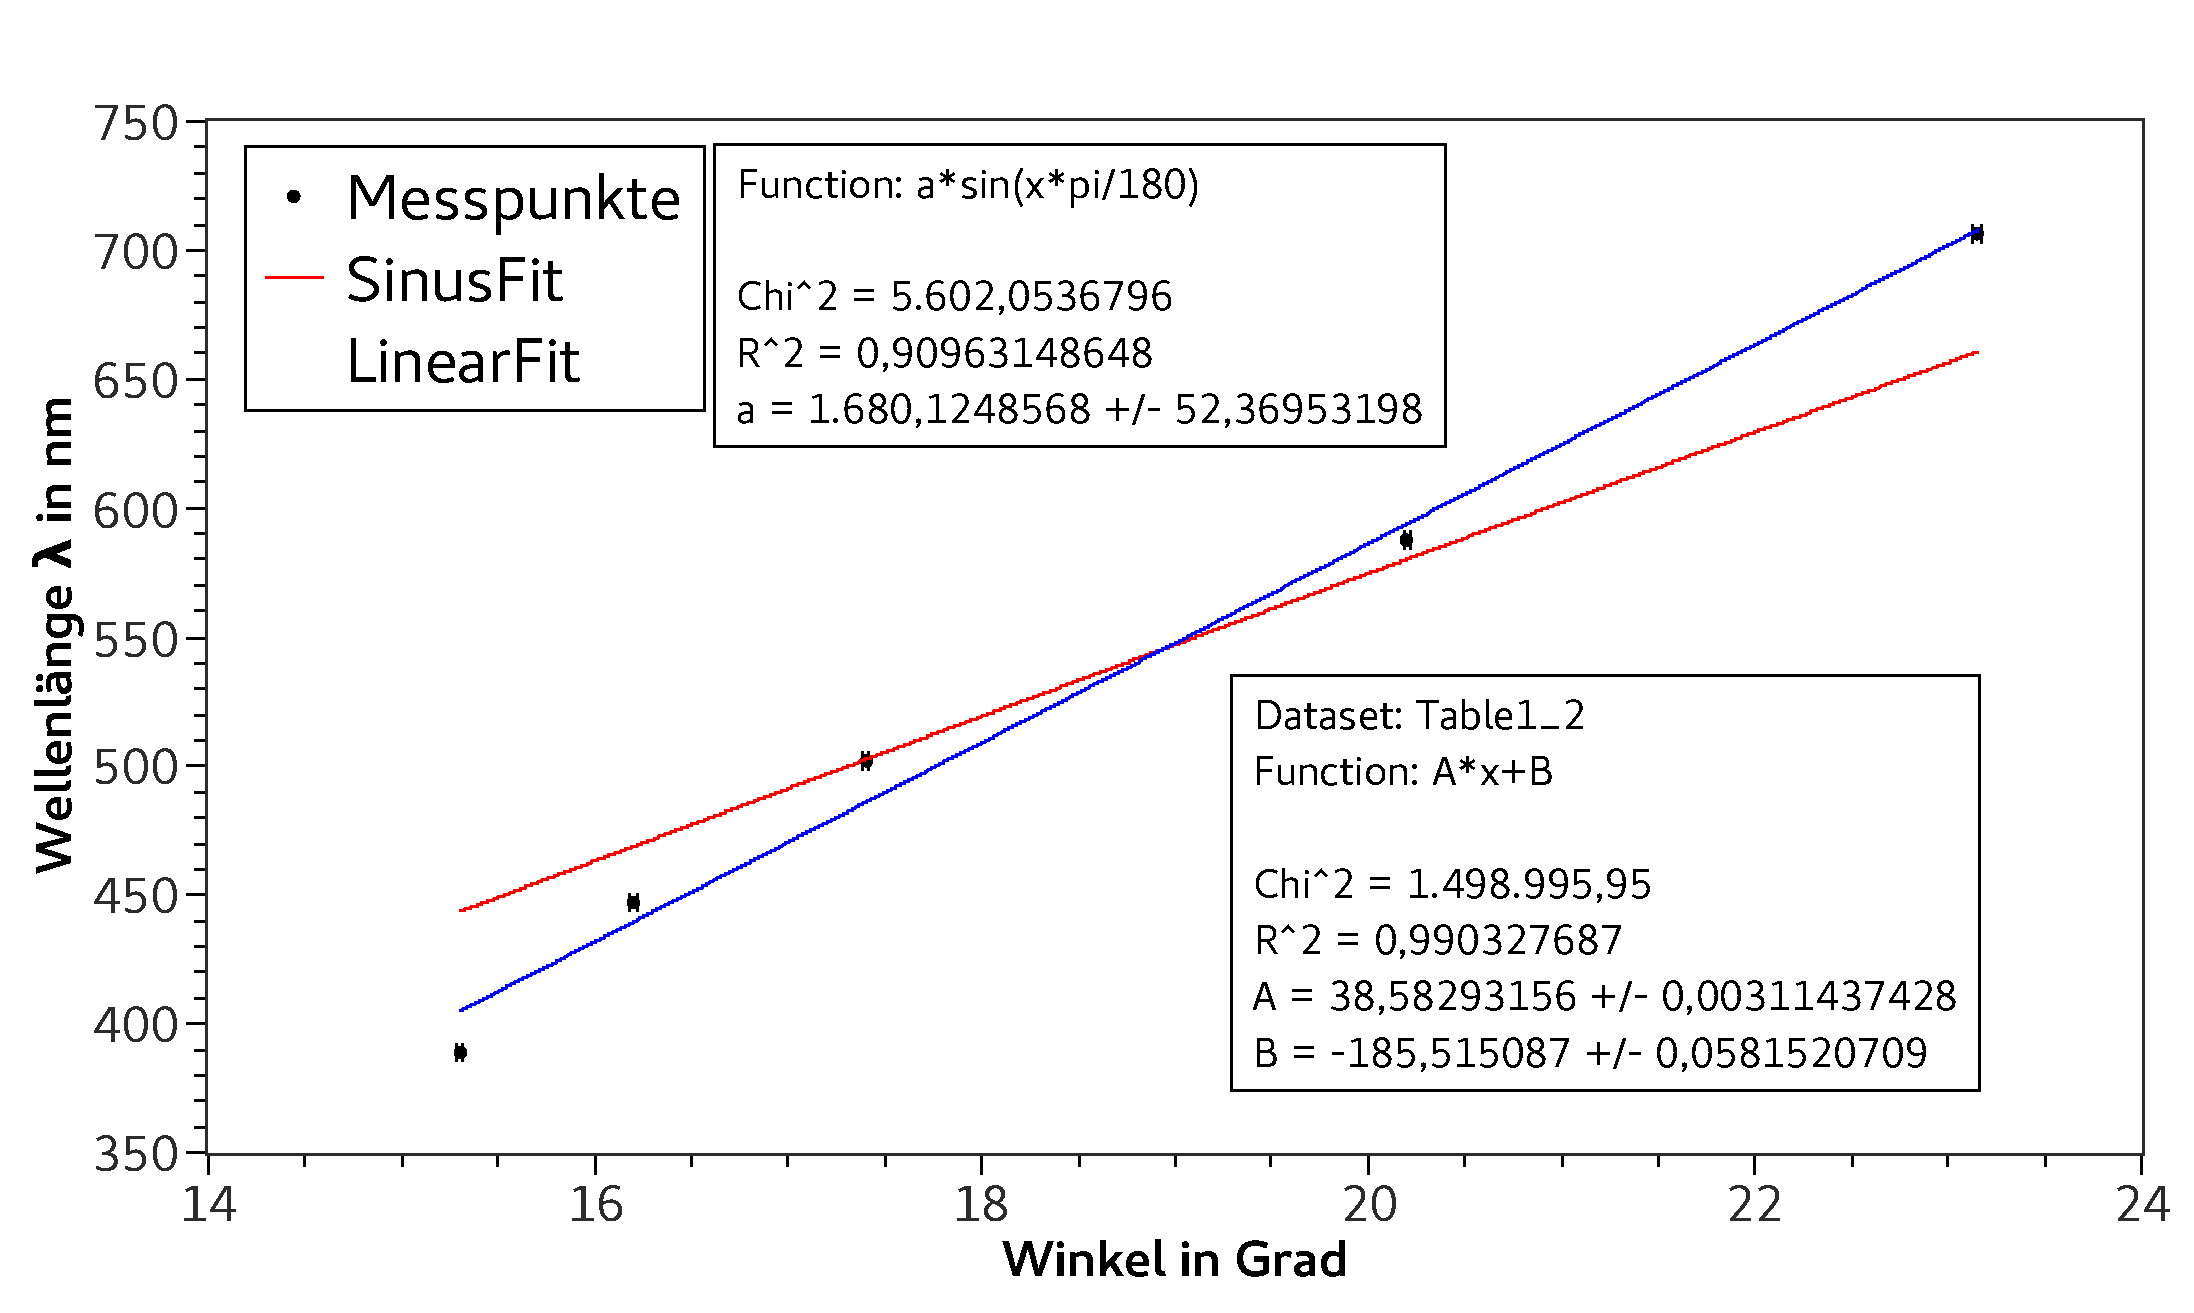
\includegraphics[width=1\textwidth]{fig_helium} 
		\centering
		\caption{Die Wellenlängen der Kalibriertabelle sind gegen die gemessenen Winkel der zugehörigen Spektrallinien aufgetragen.
		Die blaue Funktion ist ein linearer Fit.
		Die rote Funktion ist ein Sinus-Fit.
		Die sich aus den Fits ergebenden Werte $a$ bzw. $A$ sind dabei in der Einheit Nanometer bzw. Nanometer pro Grad zu verstehen.}
		\label{fig_helium}
		\centering
	\end{figure}

	\subsubsection{Diskussion}
	Die Zuordnung zur Kalibriertabelle wurde dadurch erschwert, dass das menschliche Auge bei geringen Intensitäten keine Farben mehr wahrnimmt, war aber insgesamt möglich.
	Dass einer der Messwerte sich nicht eindeutig einer Kalibrierlinie zuordnen lässt, kann an einem Messfehler beim Winkel Ablesen durch unabsichtliches Verschieben des Fernrohrs oder Ähnliches entstehen.
	
	\subsection{Energiesparlampe}
	\subsubsection{Beobachtung und Datenanalyse}
	Mithilfe der in \cref{ss_helium} bestimmten Kalibrierkurve lassen sich die Wellenlängen der Spektrallinien der Energiesparlampe ermitteln.
	Diese sind in \cref{fig_spar} dargestellt.


	\begin{figure}[H] 
		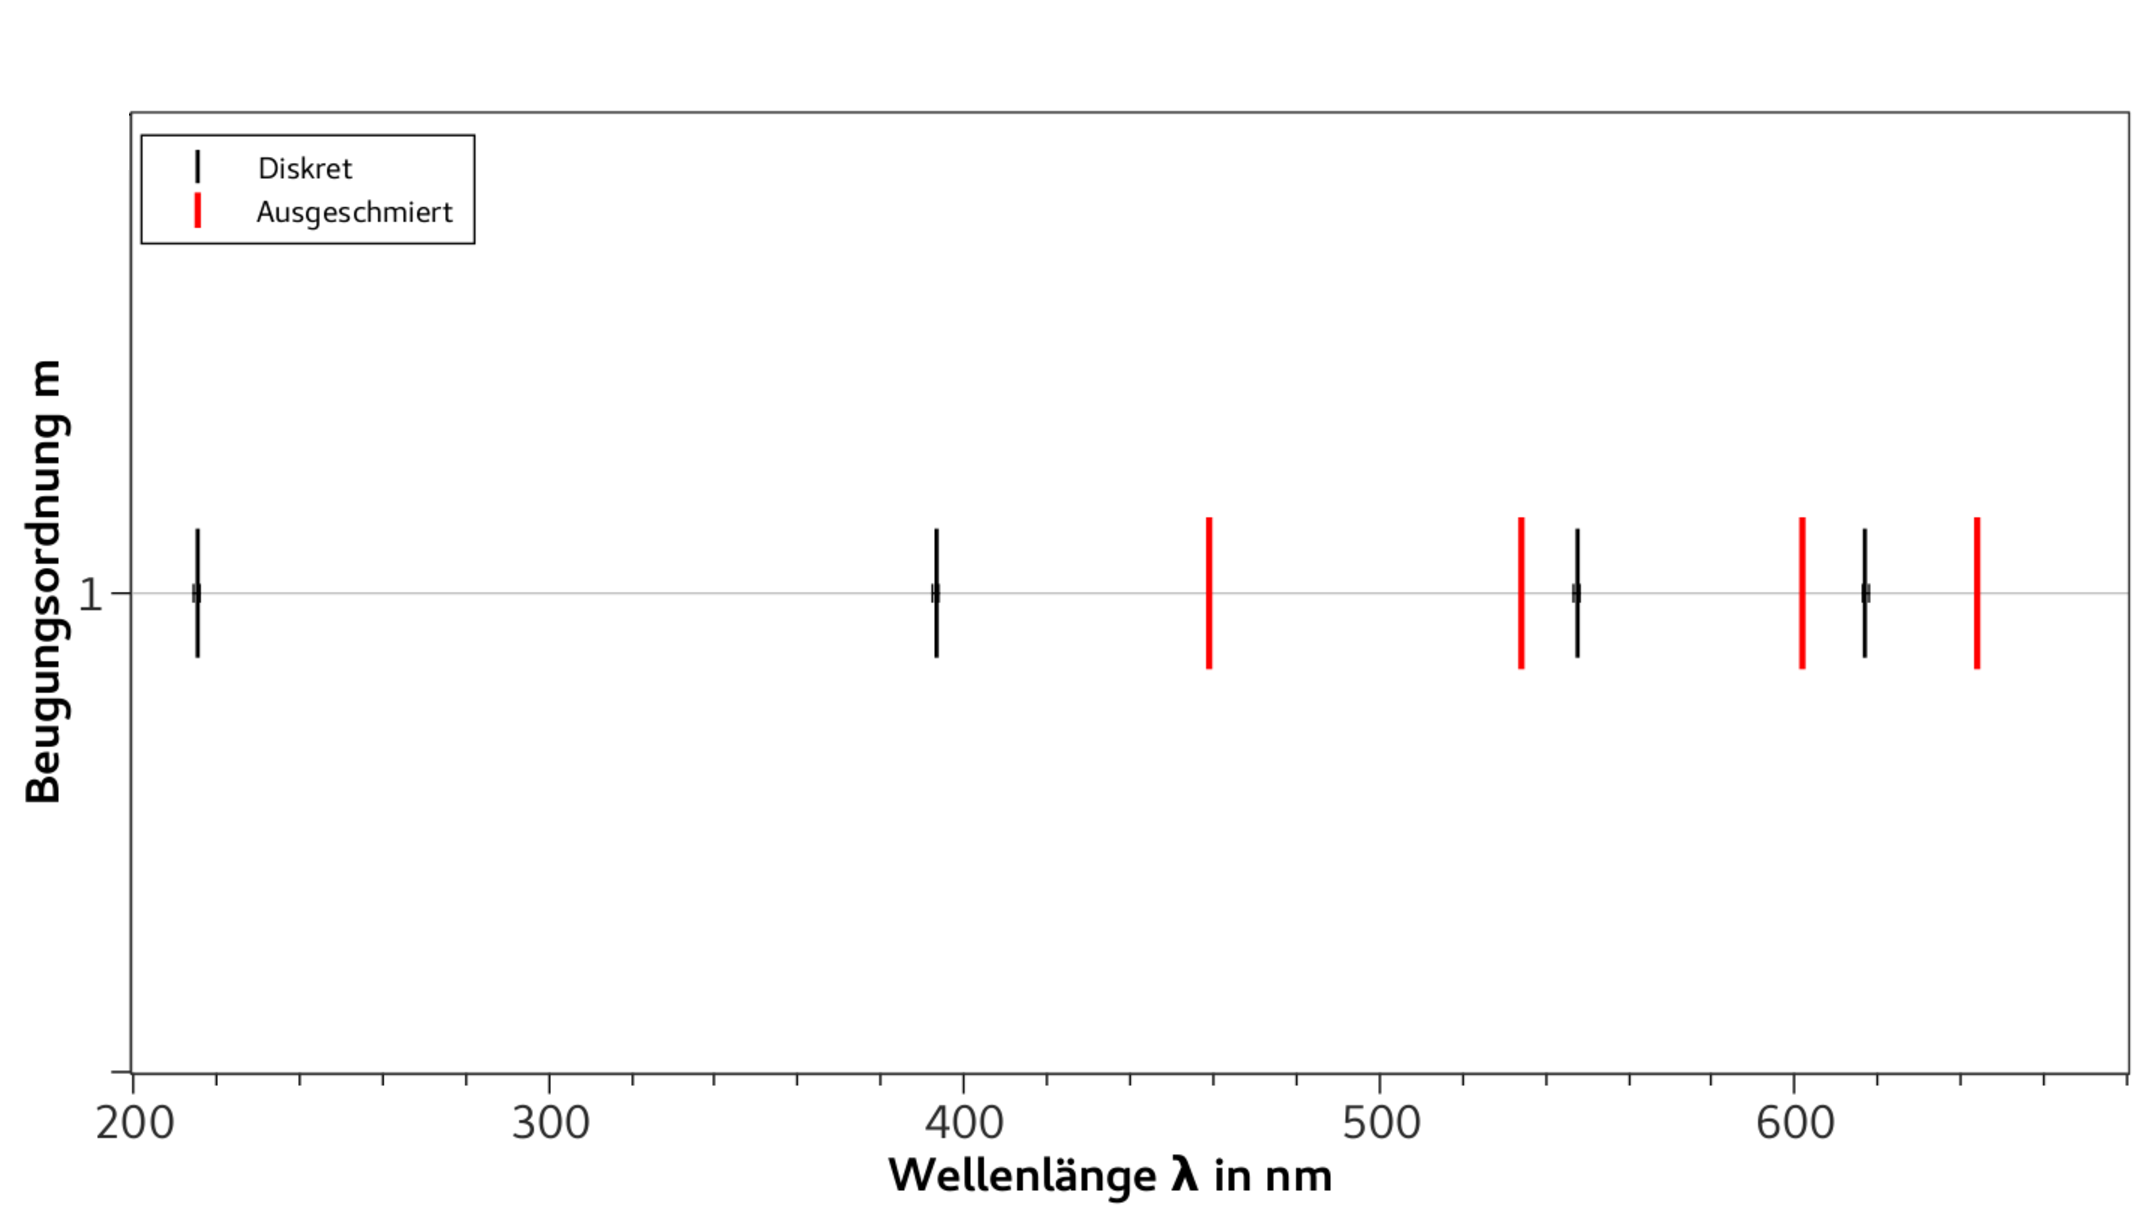
\includegraphics[width=1\textwidth]{fig_spar} 
		\centering
		\caption{Spektrallinien der Energiesparlampe.
		Es wurden lediglich Maxima der ersten Beugungsordnung beobachtet. 
		Die schwarzen Linien wurden als diskrete Spektrallinien beobachtet und die roten sind die Maxima von ausgeschmierten Spektrallinien. 
		}
		\label{fig_spar}
		\centering
	\end{figure}
	
	\subsubsection{Diskussion}
	\begin{figure}[H] 
		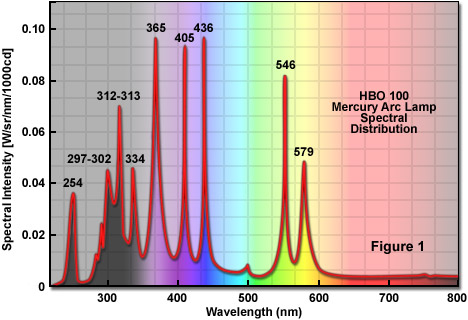
\includegraphics[width=1\textwidth]{fig_quecksilber_lit} %ist eig. mit Druck, also nicht ganz passend. tja
		\centering
		\caption{Literaturangabe nach \cite{Quecksilber} zum Spektrum von Quecksilber.}
		\label{fig_quecksilber}
		\centering
	\end{figure}

	Der Wert bei \SI{215,4}{\nano \meter} liegt im ultravioletten Bereich des elektromagnetischen Spektrums und damit außerhalb des für den Menschen sichtbaren Bereichs, weshalb er eigentlich nicht beobachtet werden können sollte.
	Dass er dennoch gemessen wird, hängt vermutlich mit dem Versagen der Näherung des Sinus als linear zusammen, da dies nur für Winkel bzw. Wellenlängen gilt, die nah an der Kalibrierkurve liegen.
	Dieser Wellenlänge liegt ein Winkel von \SI{10,4}{\degree} zugrunde, während die Messwerte für die Kalibrierkurve erst bei etwa \SI{15}{\degree} beginnen.
	Als Farbe wurde hier ein dunkles violett wahrgenommen, was dafür spricht, dass der wahre Wert der Wellenlänge am unteren Ende des sichtbaren Spektrums liegt, aber nicht im Ultravioletten.
	
	In \cref{fig_quecksilber} ist das Spektrum, das \cite{Quecksilber} für eine Quecksilberlampe angibt, dargestellt. Ein Vergleich mit den Messwerten ergibt dass die Maxima im gelben Bereich gemessen werden, wobei das eine ausgeschmiert ist. %Seite tut nur mit F5 spammen.
	Von den dreien im blauen bis ultravioletten Bereich werden nur zwei gemessen, aber da eines ausgeschmiert ist, kann ein anderes im ausgeschmierten Bereich enthalten sein.
	Außerdem werden Linien im roten Bereich gemessen, die \cite{Quecksilber} nicht angibt.
	Dies kann daran liegen, dass die Leuchtstoffröhre nicht mit einem einzelnen Gas gefüllt ist, sondern ein Gasgemisch den Leuchtstoff bildet und die Glasröhre von Innen mit einer fluoreszenten Beschichtung überzogen ist, damit ein möglichst natürlich wirkendes Licht erzeugt wird.
	
	\subsection{Leuchtdioden}
	\subsubsection{Beobachtung und Datenanalyse}
	In \cref{fig_led} wurde ein linearer Fit berechnet.  %Reihenfolge komisch, aber nicht so wichtig
	Die Energie die zum Überwinden der Bandlücke benötigt wird durch
	\begin{equation}
		E_\text{G} = eU = \frac{hc}{\lambda} 
	\end{equation}
	gegeben. 
	Es wird jedoch nicht $E_\text{G}$ sonder die Spannung $U=E/e$ aufgetragen.
	\begin{equation}
		U = \frac{hc}{e\lambda}
	\end{equation}
	Also sollte die Steigung der linearen Fits $hc/e$ entsprechen.
	Durch Division von $A$ durch $c$ lässt sich das Plancksche Wirkungsquantum als \SI{5,39 +- 0,92 e-15}{eVs} bestimmen.

	\begin{figure}[H]
		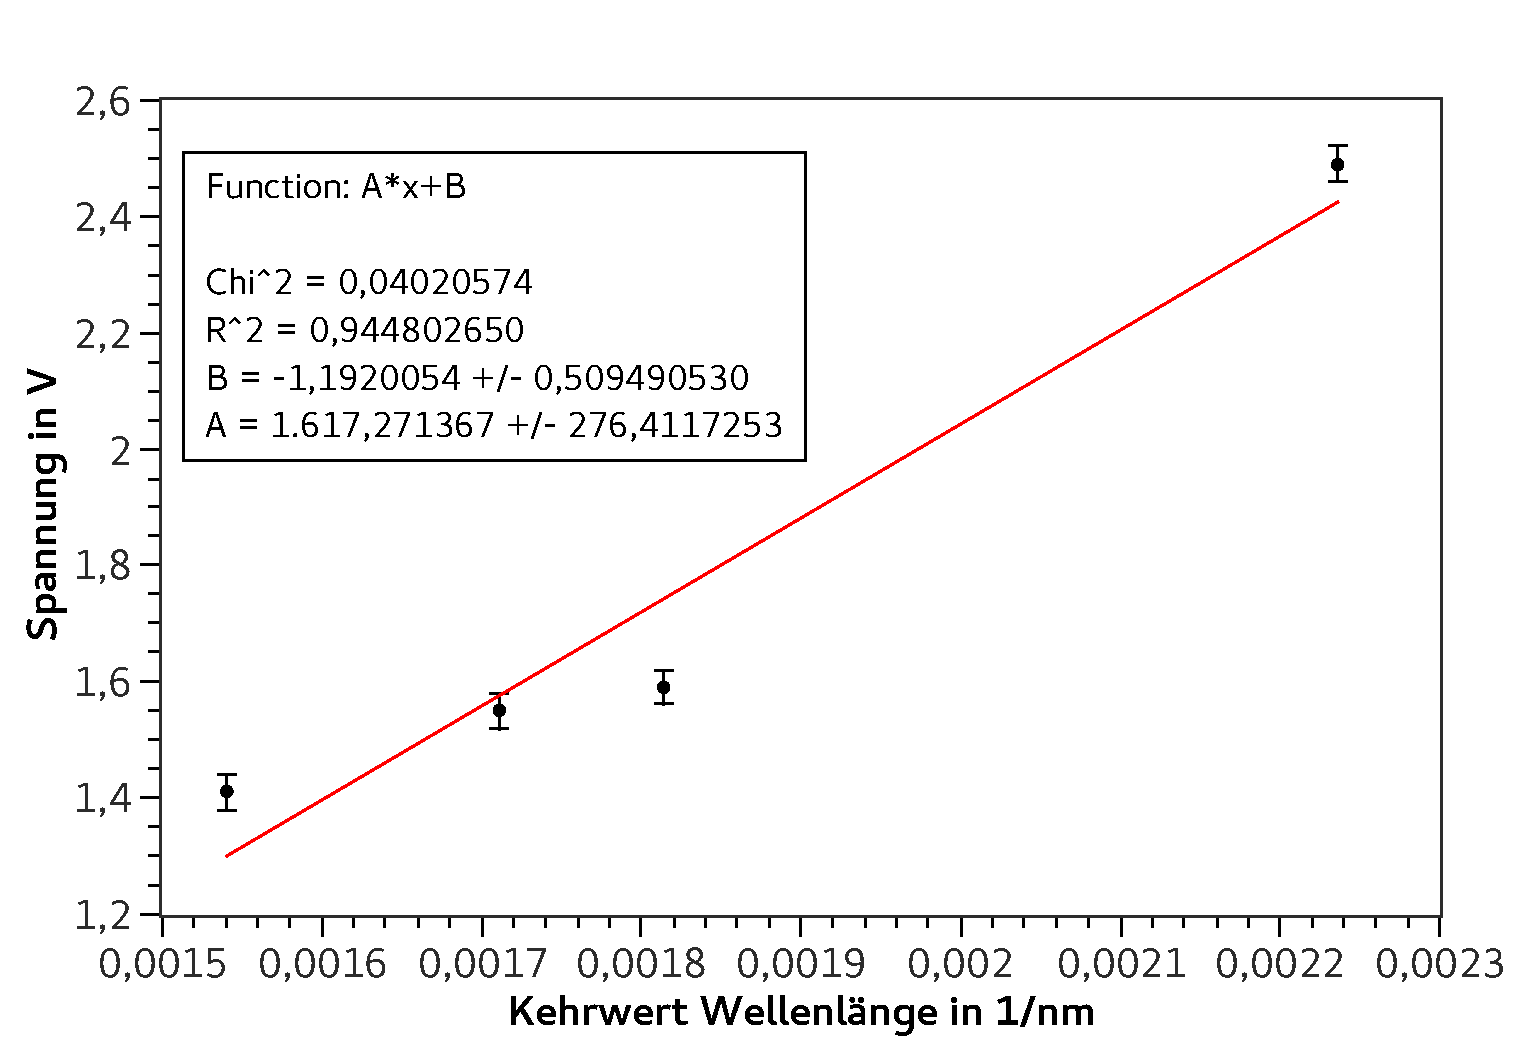
\includegraphics[width=1\textwidth]{fig_led} 
		\centering
		\caption{Die Spannung, ab der die Diode zu leuchten beginnt, ist gegen den Kehrwert des Maximums der Emissionswellenlänge aufgetragen.
		Die Emissionswellenlänge wurde aus dem Winkel des Maximums mit der Kalibrationskurve aus \cref{ss_helium} berechnet 
		Da diese Maxima nicht deutlich erkennbar waren, wurde mit einer höheren Winkelunsicherheit gerechnet.}
		\label{fig_led}
		\centering
	\end{figure}	
	
	%TODO Berechung nach Aufgabenstellung
	
	\subsubsection{Diskussion}
	
	\cite{Planck} gibt für h nach Umrechnung einen Wert von \SI{4.135667662 \pm 0.000000025}{\electronvolt \second} an.
	Dies liegt innerhalb der 1,5-fachen Unsicherheit des Messwerts.
	Da dieser jedoch bereits eine sehr große Unsicherheit hat, kann festgehalten werden, dass dies keine zielführende Methode zur Bestimmung des Planckschen Wirkungsquantums ist, aber immerhin die Bestimmung der Größenordnung erlaubt.
	Die hohe Ungenauigkeit liegt darin begründet, dass es mit dem Auge sehr schwierig ist das Emissionsmaximum präzise zu bestimmen.
	
	
	%TODO Dioden Übergänge so stochastisch, Maximum nicht sehr eindeutig zu bestimmen, keiner sagt, dass Maximum der Bandlücke entspricht, oder? Also eher Minimum der Energie bei Bandlücke?
	
	\section{Schlussfolgerung}
	Insgesamt gesehen konnten einige Feststellungen bezüglich der Messung von Spektrallinien mit dem verwendeten Spektrometer gemacht werden.
	Zunächst konnte gezeigt werden, dass sowohl ein Prisma als auch Transmissionsgitter dazu geeignet sind Licht in seine Frequenzkomponenten zu zerlegen.
	Dabei wurde jedoch festgestellt, dass keins der verwendeten Gitter eine Auflösung der Na-Doppellinie ermöglicht.
	
	Es konnte der Zusammenhang zwischen Beugungswinkel und Wellenlänge untersucht werden.
	Dabei wurde jedoch festgestellt, dass die Annahme eines linearen Zusammenhangs nur für Winkel nahe der Kalibrierkurve zu sinnvollen Ergebnissen führt, während ein sinusförmiger Zusammenhang die Messwerte nicht ausreichend widerspiegelt.
	Mit diesen Erkenntnissen wurde das Spektrum einer Energiesparlampe untersucht.
	Dabei konnte gezeigt werden, dass die Annahme es handle sich um ein einzelnes Gas nicht bestätigt werden kann und diskutiert, warum dies der Fall ist.
	
	Weiterhin wurde das Plancksche Wirkungsquantum aus den Emissionsmaxima von Leuchtdioden und der Spannung, ab der diese zu leuchten beginnen bestimmt.
	Die Annahme, dass dies mit dem Literaturwert übereinstimmt, konnte jedoch nur größenordnungsmäßig gezeigt werden.
	Um hier eine präzisere Messung zu ermöglichen wäre vorzuschlagen, mithilfe eines Photosensors die tatsächliche Intensität über das Spektrum zu messen, um daraus das Maximum der Emission deutlich exakter bestimmen zu können.
	\printbibliography
\end{document}
